% A (minimal) template for problem sets and solutions using the exam document class

% Organization:
%% Define new commands, macros, etc. in macros.tex
%% Anything that you would put before \begin{document} should go in prelude.tex

%% For multiple psets, each should get its own file to \input into main with a \section{}

\documentclass[answers, 12 pt]{exam}

\usepackage[italian]{babel}
\usepackage{graphicx}
\usepackage[utf8]{inputenc}

%% links
\usepackage{hyperref}
\hypersetup{
	colorlinks=true,
	linkcolor=blue,
	filecolor=magenta,      
	urlcolor=cyan,
	pdftitle={\titolo},
	pdfpagemode=FullScreen,
}

\graphicspath{ {./img/} }


%% configurazione per i listing di codice
\usepackage{xcolor}
\usepackage{listings}
\colorlet{mycoolgray}{gray!40}

\lstdefinestyle{output}{
	numbers=none, % where to put the line-numbers
	numberstyle=\tiny, % the size of the fonts that are used for the line-numbers     
	backgroundcolor=\color{darkgray},
	basicstyle=\ttfamily\color{white},
	captionpos=b, % sets the caption-position to bottom
	breaklines=true, % sets automatic line breaking
	breakatwhitespace=false, 
}

\lstdefinestyle{cmd}{
	numbers=none, % where to put the line-numbers
	numberstyle=\tiny, % the size of the fonts that are used for the line-numbers     
	backgroundcolor=\color{mycoolgray},
	basicstyle=\ttfamily\color{black},
	captionpos=b, % sets the caption-position to bottom
	breaklines=true, % sets automatic line breaking
	breakatwhitespace=false, 
}
\title{Esercitazione Didattica degli Elaboratori}
\begin{document}



\newcommand{\union}[2]{\underset{#1}\bigcup #2}
\newcommand{\inter}[2]{\underset{#1}\bigcap #2}

%% Compila questi campi !!

\newcommand{\esame}{Esame HPC}
\newcommand{\titolo}{Esercitazione 1 - Fedoraman}
\newcommand{\prof}{Osvaldo Gervasi}
\newcommand{\studente}{Nicolo' Vescera}

%% Content goes here

% Thesis frontmatter --------------------------------------------

\thispagestyle{empty} %suppress page number

	\noindent % just to prevent indentation narrowing the line width for this line
	
\includegraphics[width=0.15\textwidth]{img/logoUniPg}
	\begin{minipage}[b]{0.7\textwidth}
		\centering
		{\Large{\textsc{Universit{\`a} di Perugia}}}\\
		\vspace{0.4 em}
		{\large {Dipartimento di Matematica e Informatica}}
		\vspace{0.6 em}
	\end{minipage}%
	
\includegraphics[width=0.15\textwidth]{img/logoDMI}
	
	\vspace{8 em}

	\begin{center}
		

	
		{\Huge{Appunti Knowledge Representation and Automated Reasoning }}\\
		\vspace{2 em}
		{\large { Autore: Chiara Luchini}}\\
		\vspace{5 em}
		{\large {Basati su:}}\\
		{\large {- Slides del Prof. Stefano Bistarelli}}\\
		{\large {- Lezioni del Prof. Stefano Bistarelli}}\\
		%{\large \textcolor{blu_dmi}{- Appunti lezioni online Prof. Alfredo Navarra}}\\
		
	
	

%		\makebox[380pt][c]{\textcolor{blu_dmi}{\textit{Advisor} \hfill \textit{}}}
%		\makebox[380pt][c]{\textcolor{blu_dmi}{\textbf{Dott. Francesco Santini \hfill}}}
		
		\vspace{6 em}
		\vfill
		
	{\rule{380pt}{.4pt}}\\
		\vspace{1.2 em}
		\large{{Anno Accademico 2021/2022}}
		
		
		
		
	\end{center}

% ------------------------------------------------------------------
\newpage


\section{Prerequisiti}
Per questa esercitazione sono necessari i seguenti prerequisiti:

\begin{itemize}
    \item Nozioni base dell'algebra Booleana;
    \item Conoscenza e applicazione delle mappe di Karnaugh;
    \item Saper formalizzare problemi riguardanti circuiti combinatori;
    \item Saper rappresentare circuiti combinatori tramite diagrammi;
\end{itemize}

\section{Obiettivi}
Alla fine dell'esercitazione lo studente saprà interpretare il problema proposto e risolverlo con gli strumenti appresi durante il corso di Architettura degli Elaboratori. Inoltre avrà acquisito la capacità di progettare e minimizzare un circuito logico combinatorio a partire da dei dati iniziali suddividendolo in diversi passaggi fra cui:
\begin{enumerate}
    \item Definizione delle specifiche;
    \item Sintesi;
    \item Ottimizzazione;
    \item Implementazione;
    \item Verifica.
\end{enumerate}
\newpage

\section{Esercizio}
\begin{questions}
\question{
  Si chiede di progettare un sistema automatico per l'attracco di 4 navi di tipologia diversa in due differenti punti di sbarco di un porto, le quali sono individuate tramite le seguenti lettere J, C, P e S.

  Tutte quante possono arrivare contemporaneamente al porto, ma ognuna ha una diversa priorità rispetto alle altre:
    \begin{itemize}
        \item J ha una priorità maggiore di tutte le altri navi;
        \item C ha una priorità maggiore solo di P e S;
        \item P ha priorità maggiore di S.
    \end{itemize}
  Quest'ultima può essere riassunta tramite la seguente formula $J > C > P > S$. \\
  Il sistema di attracco è gestito tramite 4 differenti variabili X, Y, Z e W secondo la codifica riportata in Tabella \ref{tab:codifica}.

    \begin{table}[h!]
        \centering
            \begin{tabular}{ |p{1cm}||p{1cm}|p{1cm}|p{1cm}| p{3cm}|  }
                 \hline
                 \multicolumn{5}{|c|}{Codifica attracco navi} \\
                 \hline
                 X & Y & Z  & W& Navi\\
                 \hline
                0   & 0  &0&  0& Nessun attracco\\
                 0&   0  & 0   &1 & J\\
                 0 &0 & 1&  0 &C\\
                 0 & 1 & 0 & 0 & P\\
                 1 & 0 & 0 & 0 & S\\
                 0 & 0 & 1 & 1 &JC\\
                 0 & 1 & 0 &  1 &JP\\
                 1 & 0 & 0 &  1 &JS\\
                 0 & 1 & 1 & 0 &CP\\
                 1 & 0 & 1 &  0 &CS\\
                 1 & 1 & 0 &  0 &PS\\ 
                 \hline
            \end{tabular}

        \label{tab:codifica}
    \end{table}

}

\newpage
    \begin{solution}
       \mysection{Formulazione}
        Creazione della tabella di verità.
        
            \begin{center}
              \begin{tabular}{cccc|cccc|c}
                J & C & P & S & X & Y & Z & W & Attracco\\
                \hline
                0 & 0 & 0 &0 & 0 & 0 & 0 &0 & Nessuna\\
                0 & 0 & 0 &1 & 1 & 0 & 0 &0 & S\\
                0 & 0 & 1 & 0 & 0 & 1 & 0 & 0 & P\\
                0 & 0 & 1 & 1 & 1 & 1 & 0 & 0 & PS \\
                0 & 1 & 0 & 0 & 0 & 0 & 1 & 0 & C \\ 
                0 & 1 & 0 & 1 & 1 & 0 & 1 & 0 & CS \\
                0 & 1 & 1 & 0 & 0 & 1 & 1 & 0 & CP \\
                0 & 1 & 1 & 1 & 0 & 1 & 1 & 0 & CP \\
                1 & 0 & 0 & 0 & 0 & 0 & 0 & 1 & J \\
                1 & 0 & 0 & 1 & 1 & 0 & 0 & 1 & JS \\
                1 & 0 & 1 & 0 & 0 & 1 & 0 & 1 & JP \\
                1 & 0 & 1 & 1 & 0 & 1 & 0 & 1 & JP \\
                1 & 1 & 0 & 0 & 0 & 0 & 1 & 1 & JC \\
                1 & 1 & 0 & 1 & 0 & 0 & 1 & 1 & JC \\
                1 & 1 & 1 & 0 & 0 & 0 & 1 & 1 & JC \\
                1 & 1 & 1 & 1 & 0 & 0 & 1 & 1 & JC\\
              \end{tabular}
            \end{center}
            
        \mysection{Ottimizzazione}
            Creazione delle Mappe di Karnaugh.
            \begin{enumerate}
                    \item Mappa di Karnaugh per X.
                    
                        \begin{center}
                            \begin{karnaugh-map}[4][4][1][$JC$][$PS$]
                                \manualterms{0,0,0,0,1,1,1,0,0,0,0,0,1,0,0,0}
                                \implicant{4}{12}
                                \implicant{4}{5}
                                \implicantedge{4}{4}{6}{6}
                             \end{karnaugh-map}
                        \end{center}
                        \[ X = S \overline{CP}  +  S \overline{JP} + S \overline{JC}  \]
                        
                    \item Mappa di Karnaugh per Y.
                    
                        \begin{center}
                            \begin{karnaugh-map}[4][4][1][$JC$][$PS$]
                                \manualterms{0,0,0,0,0,0,0,0,1,1,1,0,1,1,1,0}
                                \implicant{12}{9}
                                \implicantedge{12}{8}{14}{10}
                             \end{karnaugh-map}
                        \end{center}
                    \[ Y = P \overline{J}  +  P \overline{C} \]
                    
                     \item Mappa di Karnaugh per Z.
                    
                        \begin{center}
                            \begin{karnaugh-map}[4][4][1][$JC$][$PS$]
                                \manualterms{0,1,0,1,0,1,0,1,0,1,0,1,0,1,0,1}
                                \implicant{1}{11}
                             \end{karnaugh-map}
                        \end{center}
                    \[ Z = C \]
                    
                    
                    \item Mappa di Karnaugh per W.
                    
                        \begin{center}
                            \begin{karnaugh-map}[4][4][1][$JC$][$PS$]
                                \manualterms{0,0,1,1,0,0,1,1,0,0,1,1,0,0,1,1}
                                \implicant{3}{10}
                             \end{karnaugh-map}
                        \end{center}
                    \[ W = J \]
            \end{enumerate}
            
            \mysection{Disegno del circuito}
            Disegno del circuito combinatorio non minimizzato.
             %%%%%%%%%%%%  DA FARE %%%%%%%%%%%%%
                    \begin{center}
                        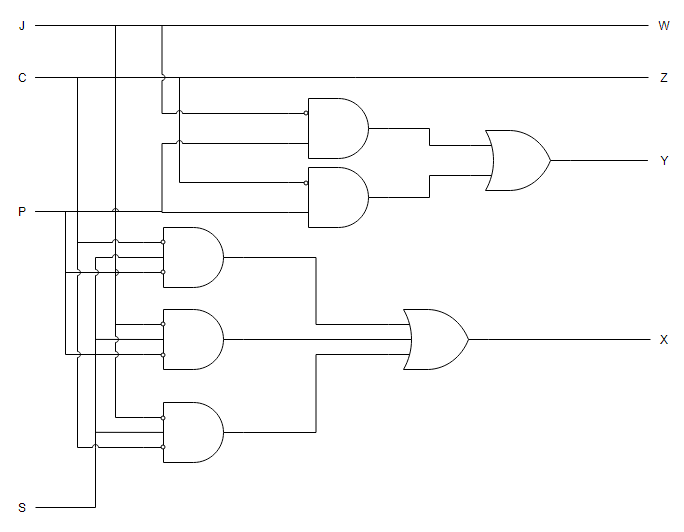
\includegraphics[width=13cm, keepaspectratio]{img/carpi_diagramma_no_min.png}
                    \end{center}
            \newpage
            Disegno del circuito combinatorio minimizzato tramite le seguenti formule:    
                \[ X = S(\overline{CP} + \overline{JP} + \overline{JC})\]
                \[ Y = P(\overline{J} +\overline{C})\]
                \[ Z = C \]
                \[ W = J \]
                    \begin{center}
                            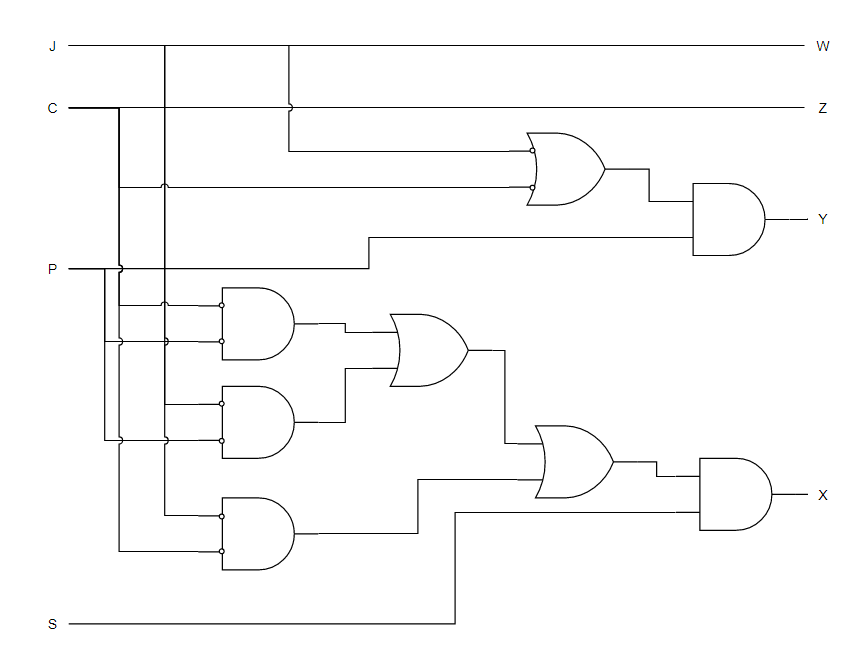
\includegraphics[width=13cm, keepaspectratio]{img/carpi_diagramma.png}
                    \end{center}
                 

    \end{solution}
\end{questions}


\end{document}